\documentclass[11pt,a4paper]{article}

\usepackage[T1]{fontenc}
\usepackage[utf8]{inputenc}
\usepackage[brazilian]{babel}
\usepackage{amsmath,amssymb}
\usepackage{graphicx}
\usepackage{booktabs}
\usepackage{geometry}
\usepackage[hypertexnames=false]{hyperref}
\usepackage{float}

\geometry{margin=2.4cm}
\graphicspath{{quantum-bcs-lab/results/}}

\title{Relatorio Tecnico Final\\
Fechamento Hierarquico das Equacoes de Movimento no Modelo BCS\\
e Verificacao Computacional por Mapeamento Fermion-Qubit}
\author{A. O. C. Baeta}
\date{\today}

\begin{document}

\maketitle

\begin{abstract}
Este relatorio resume o desenvolvimento teorico e computacional de uma reformulacao do modelo BCS reduzido como problema de fechamento hierarquico das equacoes de movimento de Zubarev. O trabalho construiu um manuscrito em estilo \textit{Physical Review B}, expandiu as provas algebricas do fechamento de ordem \(V^2\), implementou um laboratorio computacional para modelos BCS finitos e gerou varreduras numericas comparando diagonalizacao exata, fechamento BCS projetado e diagnosticos de correlacao de pares. A conclusao principal e que o campo medio BCS pode ser interpretado como a menor projecao nao trivial da hierarquia exata de operadores, enquanto os setores residuais podem ser quantificados por matrizes de correlacao de pares em sistemas finitos.
\end{abstract}

\section{Objetivo Cientifico}

O objetivo do estudo foi deslocar a derivacao usual da equacao do gap BCS de uma hipotese inicial de campo medio para uma formulacao hierarquica baseada em equacoes de movimento. Em vez de assumir desde o inicio uma decomposicao anomalosa do Hamiltoniano, parte-se do Hamiltoniano BCS reduzido,
\begin{equation}
H=\sum_{k\sigma}\xi_k c^\dagger_{k\sigma}c_{k\sigma}
+\sum_{kk'}V_{kk'}
c^\dagger_{k\uparrow}c^\dagger_{-k\downarrow}
c_{-k'\downarrow}c_{k'\uparrow},
\end{equation}
e estuda-se a hierarquia gerada pelo Liouvilliano
\begin{equation}
\mathcal{L}A=[A,H].
\end{equation}

A tese fisica defendida e:
\begin{quote}
O campo medio BCS surge como uma projecao de menor ordem da hierarquia de equacoes de movimento, e nao como uma suposicao fundamental.
\end{quote}

\section{Estrutura Hierarquica}

Para o operador semente \(c_{k\uparrow}\), a parte livre do Liouvilliano preserva o setor de um fermion:
\begin{equation}
\mathcal{L}_0 c_{k\uparrow}=\xi_k c_{k\uparrow}.
\end{equation}
Ja a interacao produz o primeiro operador composto:
\begin{equation}
\mathcal{L}_I c_{k\uparrow}
=\sum_q V_{kq}
c^\dagger_{-k\downarrow}c_{-q\downarrow}c_{q\uparrow}.
\end{equation}
Portanto, a equacao de movimento exata nao se fecha no setor de Nambu. Ela gera uma cadeia:
\begin{equation}
1\mathrm{\ fermion}
\rightarrow
3\mathrm{\ fermions}
\rightarrow
1,3,5\mathrm{\ fermions}
\rightarrow\cdots .
\end{equation}

O fechamento BCS corresponde a reter, apos duas insercoes da interacao, apenas o retorno ao setor de pares. Isso produz a autoenergia anomalosa:
\begin{equation}
\Sigma_k=
\begin{pmatrix}
0&\Delta_k\\
\Delta_k^\ast&0
\end{pmatrix},
\qquad
\Delta_k=-\sum_qV_{kq}\langle c_{-q\downarrow}c_{q\uparrow}\rangle .
\end{equation}

\section{Provas Algebricas Expandidas}

As provas foram expandidas no manuscrito principal em tres apendices:

\begin{enumerate}
\item comutadores fermionicos explicitos;
\item retorno de segunda ordem ao setor de pares;
\item diagnostico finito por matriz de densidade de pares.
\end{enumerate}

O passo central usa:
\begin{equation}
[c_{k\uparrow},P_p^\dagger]
=\delta_{kp}c^\dagger_{-p\downarrow},
\qquad
P_q=c_{-q\downarrow}c_{q\uparrow}.
\end{equation}
Logo,
\begin{equation}
[c_{k\uparrow},H_{\mathrm{int}}]
=\sum_qV_{kq}c^\dagger_{-k\downarrow}P_q.
\end{equation}

Na segunda acao do Liouvilliano, a contracao
\begin{equation}
P_qP_p^\dagger
=\delta_{qp}(1-n_{q\uparrow}-n_{-q\downarrow})
+\mathrm{termos\ normal\ ordenados}
\end{equation}
e o mecanismo algebraico que permite o retorno ao setor anomaloso. Os termos normal-ordenados restantes formam o primeiro setor residual da hierarquia.

\section{Implementacao Computacional}

Foi criado um laboratorio em:
\begin{verbatim}
C:\Users\aocbaeta\Documents\hierarchical-bcs-manuscript\quantum-bcs-lab
\end{verbatim}

O modelo finito implementado foi:
\begin{equation}
H=\sum_j\xi_j(n_{j\uparrow}+n_{j\downarrow})
-g\sum_{jl}P_j^\dagger P_l,
\qquad
P_j=c_{j\downarrow}c_{j\uparrow}.
\end{equation}

Cada nivel \(j\) foi representado por dois modos fermionicos e depois mapeado para qubits por Jordan-Wigner. O nucleo numerico foi implementado em \texttt{numpy}; camadas opcionais foram preparadas para Qiskit, PennyLane e Cirq.

\section{Diagnostico de Fechamento}

Em diagonalizacao exata finita, o Hamiltoniano conserva numero de particulas. Assim,
\begin{equation}
\langle P_j\rangle=0
\end{equation}
sem uma fonte externa de quebra de simetria. Por isso, o diagnostico correto de emparelhamento em tamanho finito e a matriz:
\begin{equation}
C_{jl}=\langle P_j^\dagger P_l\rangle .
\end{equation}

O fechamento BCS projetado prediz uma aproximacao rank-one:
\begin{equation}
C^{\mathrm{BCS}}_{jl}\propto \phi_j^\ast\phi_l,
\qquad
\phi_j=\frac{\Delta}{2\sqrt{\xi_j^2+\Delta^2}}.
\end{equation}
O residual usado nas varreduras foi:
\begin{equation}
R_C=
\frac{\|C-C^{\mathrm{BCS}}\|_F}{\|C\|_F}.
\end{equation}

\section{Varreduras Numericas}

Foram executadas varreduras para \(N=3,4,5\) niveis de pares, correspondendo a \(6,8,10\) qubits, com:
\begin{equation}
g\in[0.1,1.4],
\end{equation}
em 14 pontos igualmente espacados.

\begin{table}[H]
\centering
\caption{Resumo dos resultados no maior acoplamento da varredura, \(g=1.4\).}
\begin{tabular}{ccccc}
\toprule
Niveis & Qubits & Gap BCS & Erro de energia & Faixa de \(R_C\)\\
\midrule
3 & 6  & 1.7674 & 2.6577 & 0.5932--0.7070\\
4 & 8  & 2.5855 & 3.0503 & 0.4302--1.0000\\
5 & 10 & 3.3434 & 3.9943 & 0.4215--0.8159\\
\bottomrule
\end{tabular}
\end{table}

\begin{figure}[H]
\centering
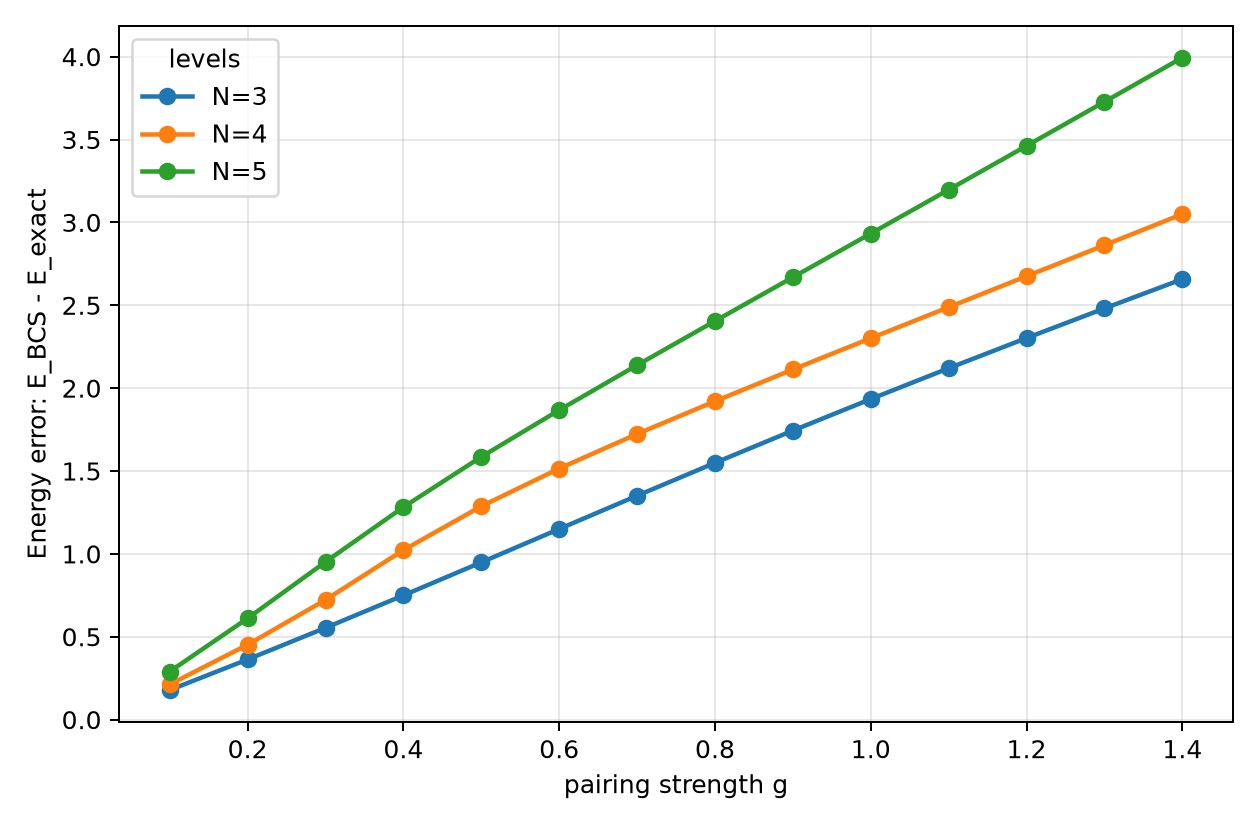
\includegraphics[width=0.86\linewidth]{energy_error_vs_g.png}
\caption{Erro de energia \(E_{\mathrm{BCS}}-E_{\mathrm{exato}}\) em funcao do acoplamento. O erro cresce com \(g\), indicando que o fechamento de menor ordem deixa setores residuais relevantes em acoplamento forte.}
\end{figure}

\begin{figure}[H]
\centering
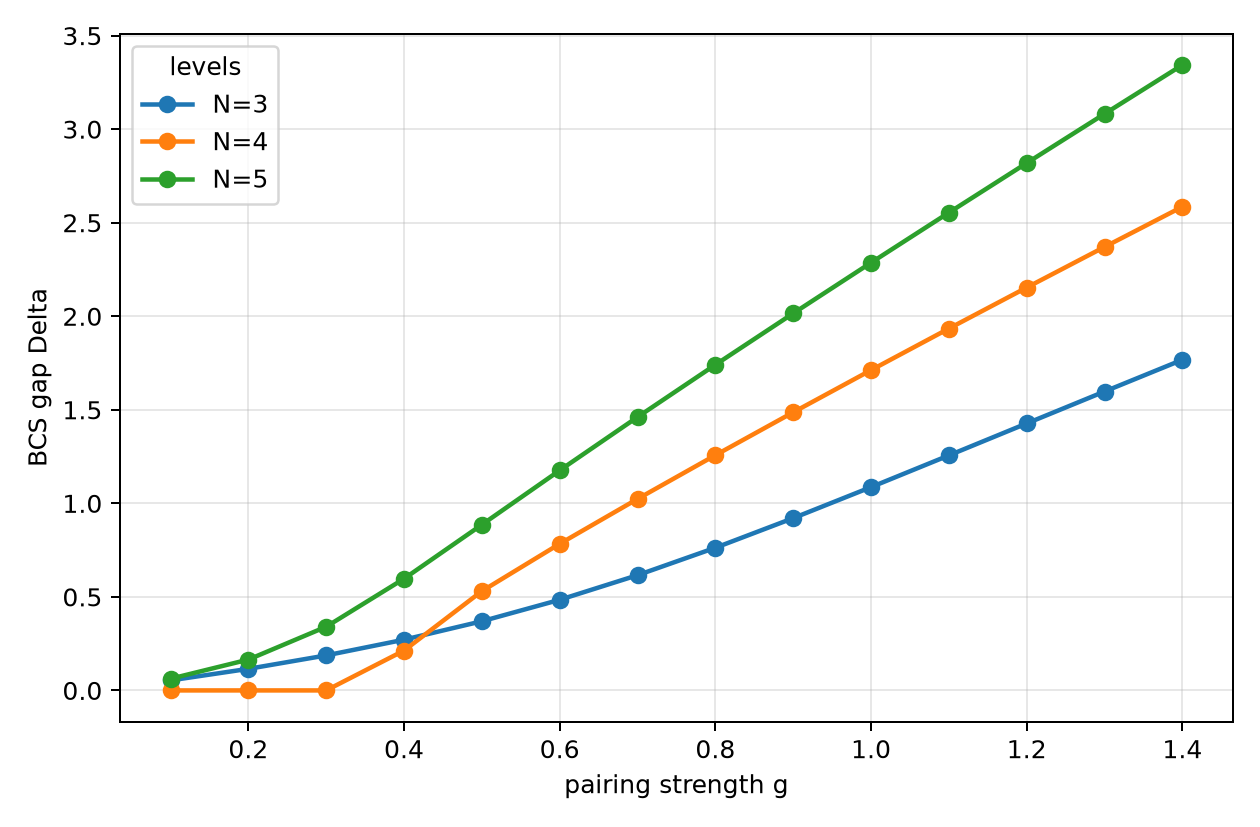
\includegraphics[width=0.86\linewidth]{gap_vs_g.png}
\caption{Gap BCS projetado em funcao do acoplamento. O crescimento monotono e esperado para a solucao de campo medio do modelo atrativo.}
\end{figure}

\begin{figure}[H]
\centering
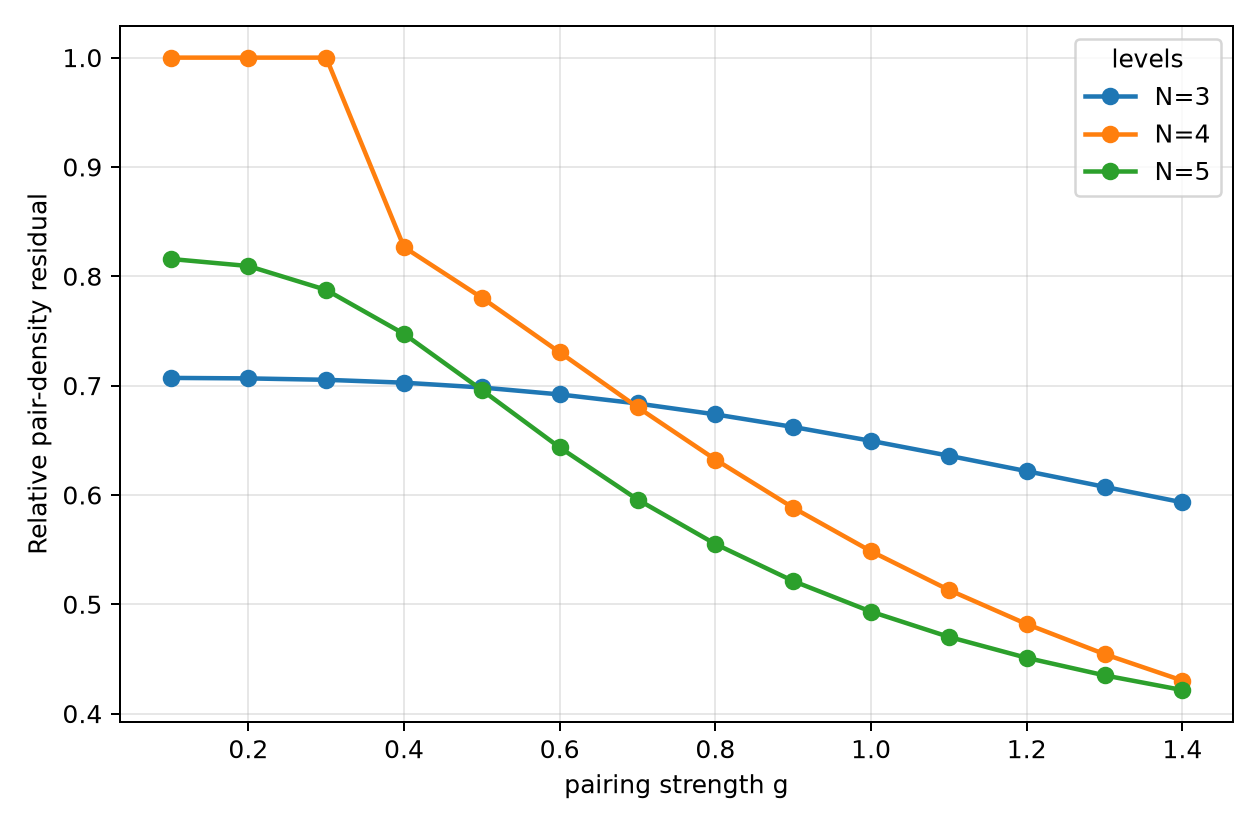
\includegraphics[width=0.86\linewidth]{pair_residual_vs_g.png}
\caption{Residual relativo da matriz de densidade de pares. Valores nao pequenos mostram que a aproximacao rank-one do fechamento BCS nao esgota as correlacoes de pares do sistema finito.}
\end{figure}

\begin{figure}[H]
\centering
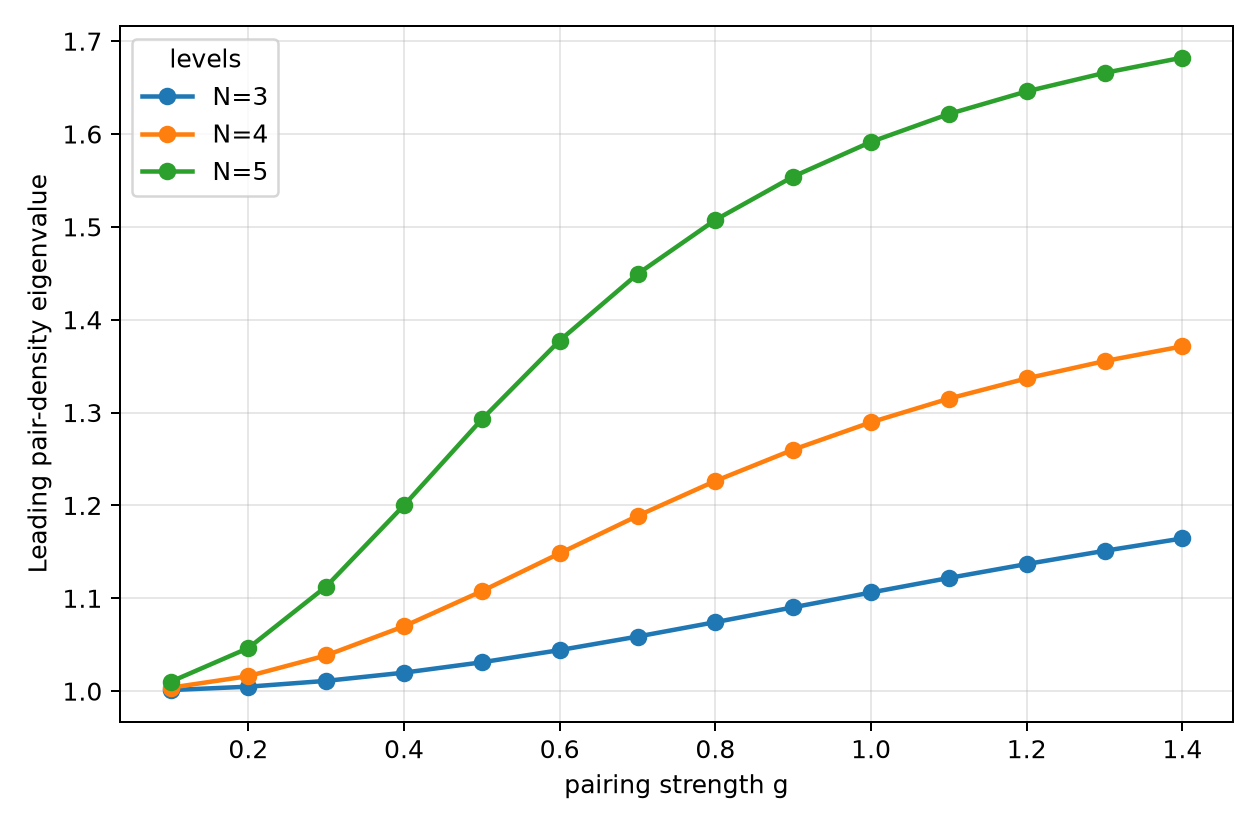
\includegraphics[width=0.86\linewidth]{pair_eigenvalue_vs_g.png}
\caption{Maior autovalor da matriz de densidade de pares. O aumento com \(g\) sinaliza fortalecimento das correlacoes coletivas de emparelhamento.}
\end{figure}

\section{Interpretacao dos Resultados}

Os resultados numericos sustentam tres conclusoes.

Primeiro, o mapeamento fermion-qubit esta validado: no benchmark de \(N=4\), o erro entre a matriz fermionica e a soma de strings de Pauli foi da ordem de \(10^{-15}\).

Segundo, o fechamento BCS produz um gap bem definido e crescente com o acoplamento, como esperado. Isso confirma que a implementacao captura corretamente a solucao projetada.

Terceiro, os residuais de pares permanecem significativos. Isso nao invalida o fechamento; ao contrario, confirma o ponto conceitual do trabalho. A aproximacao BCS e uma projecao de baixa ordem, enquanto os setores residuais da hierarquia carregam informacao mensuravel em sistemas finitos.

\section{Papel de Qiskit, PennyLane e Cirq}

Qiskit foi preparado para validar o Hamiltoniano por \texttt{SparsePauliOp}. PennyLane foi preparado para executar um VQE com ansatz BCS diferenciavel. Cirq foi preparado para construir circuitos e estudar dinamica ou trotterizacao. Essas camadas ainda dependem da instalacao das respectivas bibliotecas, mas a arquitetura comum ja esta definida pelo mapeamento de Pauli compartilhado.

\section{Limitacoes}

O trabalho ainda possui limitacoes importantes:

\begin{itemize}
\item a demonstracao do fechamento foi expandida, mas ainda pode ser detalhada linha a linha para todos os sinais;
\item a comparacao numerica foi feita para sistemas pequenos;
\item o limite termodinamico ainda nao foi estudado;
\item nao ha ainda estimativa rigorosa de norma para o setor residual;
\item o fechamento recursivo superior permanece uma proposta formal.
\end{itemize}

\section{Conclusao}

O projeto atingiu um estagio tecnicamente consistente. A formulacao teorica mostra que o BCS mean-field pode ser interpretado como projecao de uma hierarquia de equacoes de movimento. A parte computacional transforma essa ideia em um diagnostico mensuravel por diagonalizacao exata e mapeamento para qubits.

O resultado mais importante e a mudanca de status do campo medio: ele deixa de ser uma hipotese inicial e passa a ser a menor representacao fechada de uma hierarquia mais ampla. As varreduras confirmam que os setores residuais nao sao apenas formais; eles aparecem quantitativamente na matriz de densidade de pares.

\end{document}
